\documentclass[1p]{elsarticle_modified}
%\bibliographystyle{elsarticle-num}

%\usepackage[colorlinks]{hyperref}
%\usepackage{abbrmath_seonhwa} %\Abb, \Ascr, \Acal ,\Abf, \Afrak
\usepackage{amsfonts}
\usepackage{amssymb}
\usepackage{amsmath}
\usepackage{amsthm}
\usepackage{scalefnt}
\usepackage{amsbsy}
\usepackage{kotex}
\usepackage{caption}
\usepackage{subfig}
\usepackage{color}
\usepackage{graphicx}
\usepackage{xcolor} %% white, black, red, green, blue, cyan, magenta, yellow
\usepackage{float}
\usepackage{setspace}
\usepackage{hyperref}

\usepackage{tikz}
\usetikzlibrary{arrows}

\usepackage{multirow}
\usepackage{array} % fixed length table
\usepackage{hhline}

%%%%%%%%%%%%%%%%%%%%%
\makeatletter
\renewcommand*\env@matrix[1][\arraystretch]{%
	\edef\arraystretch{#1}%
	\hskip -\arraycolsep
	\let\@ifnextchar\new@ifnextchar
	\array{*\c@MaxMatrixCols c}}
\makeatother %https://tex.stackexchange.com/questions/14071/how-can-i-increase-the-line-spacing-in-a-matrix
%%%%%%%%%%%%%%%

\usepackage[normalem]{ulem}

\newcommand{\msout}[1]{\ifmmode\text{\sout{\ensuremath{#1}}}\else\sout{#1}\fi}
%SOURCE: \msout is \stkout macro in https://tex.stackexchange.com/questions/20609/strikeout-in-math-mode

\newcommand{\cancel}[1]{
	\ifmmode
	{\color{red}\msout{#1}}
	\else
	{\color{red}\sout{#1}}
	\fi
}

\newcommand{\add}[1]{
	{\color{blue}\uwave{#1}}
}

\newcommand{\replace}[2]{
	\ifmmode
	{\color{red}\msout{#1}}{\color{blue}\uwave{#2}}
	\else
	{\color{red}\sout{#1}}{\color{blue}\uwave{#2}}
	\fi
}

\newcommand{\Sol}{\mathcal{S}} %segment
\newcommand{\D}{D} %diagram
\newcommand{\A}{\mathcal{A}} %arc


%%%%%%%%%%%%%%%%%%%%%%%%%%%%%5 test

\def\sl{\operatorname{\textup{SL}}(2,\Cbb)}
\def\psl{\operatorname{\textup{PSL}}(2,\Cbb)}
\def\quan{\mkern 1mu \triangleright \mkern 1mu}

\theoremstyle{definition}
\newtheorem{thm}{Theorem}[section]
\newtheorem{prop}[thm]{Proposition}
\newtheorem{lem}[thm]{Lemma}
\newtheorem{ques}[thm]{Question}
\newtheorem{cor}[thm]{Corollary}
\newtheorem{defn}[thm]{Definition}
\newtheorem{exam}[thm]{Example}
\newtheorem{rmk}[thm]{Remark}
\newtheorem{alg}[thm]{Algorithm}

\newcommand{\I}{\sqrt{-1}}
\begin{document}

%\begin{frontmatter}
%
%\title{Boundary parabolic representations of knots up to 8 crossings}
%
%%% Group authors per affiliation:
%\author{Yunhi Cho} 
%\address{Department of Mathematics, University of Seoul, Seoul, Korea}
%\ead{yhcho@uos.ac.kr}
%
%
%\author{Seonhwa Kim} %\fnref{s_kim}}
%\address{Center for Geometry and Physics, Institute for Basic Science, Pohang, 37673, Korea}
%\ead{ryeona17@ibs.re.kr}
%
%\author{Hyuk Kim}
%\address{Department of Mathematical Sciences, Seoul National University, Seoul 08826, Korea}
%\ead{hyukkim@snu.ac.kr}
%
%\author{Seokbeom Yoon}
%\address{Department of Mathematical Sciences, Seoul National University, Seoul, 08826,  Korea}
%\ead{sbyoon15@snu.ac.kr}
%
%\begin{abstract}
%We find all boundary parabolic representation of knots up to 8 crossings.
%
%\end{abstract}
%\begin{keyword}
%    \MSC[2010] 57M25 
%\end{keyword}
%
%\end{frontmatter}

%\linenumbers
%\tableofcontents
%
\newcommand\colored[1]{\textcolor{white}{\rule[-0.35ex]{0.8em}{1.4ex}}\kern-0.8em\color{red} #1}%
%\newcommand\colored[1]{\textcolor{white}{ #1}\kern-2.17ex	\textcolor{white}{ #1}\kern-1.81ex	\textcolor{white}{ #1}\kern-2.15ex\color{red}#1	}

{\Large $\underline{12n_{0529}~(K12n_{0529})}$}

\setlength{\tabcolsep}{10pt}
\renewcommand{\arraystretch}{1.6}
\vspace{1cm}\begin{tabular}{m{100pt}>{\centering\arraybackslash}m{274pt}}
\multirow{5}{120pt}{
	\centering
	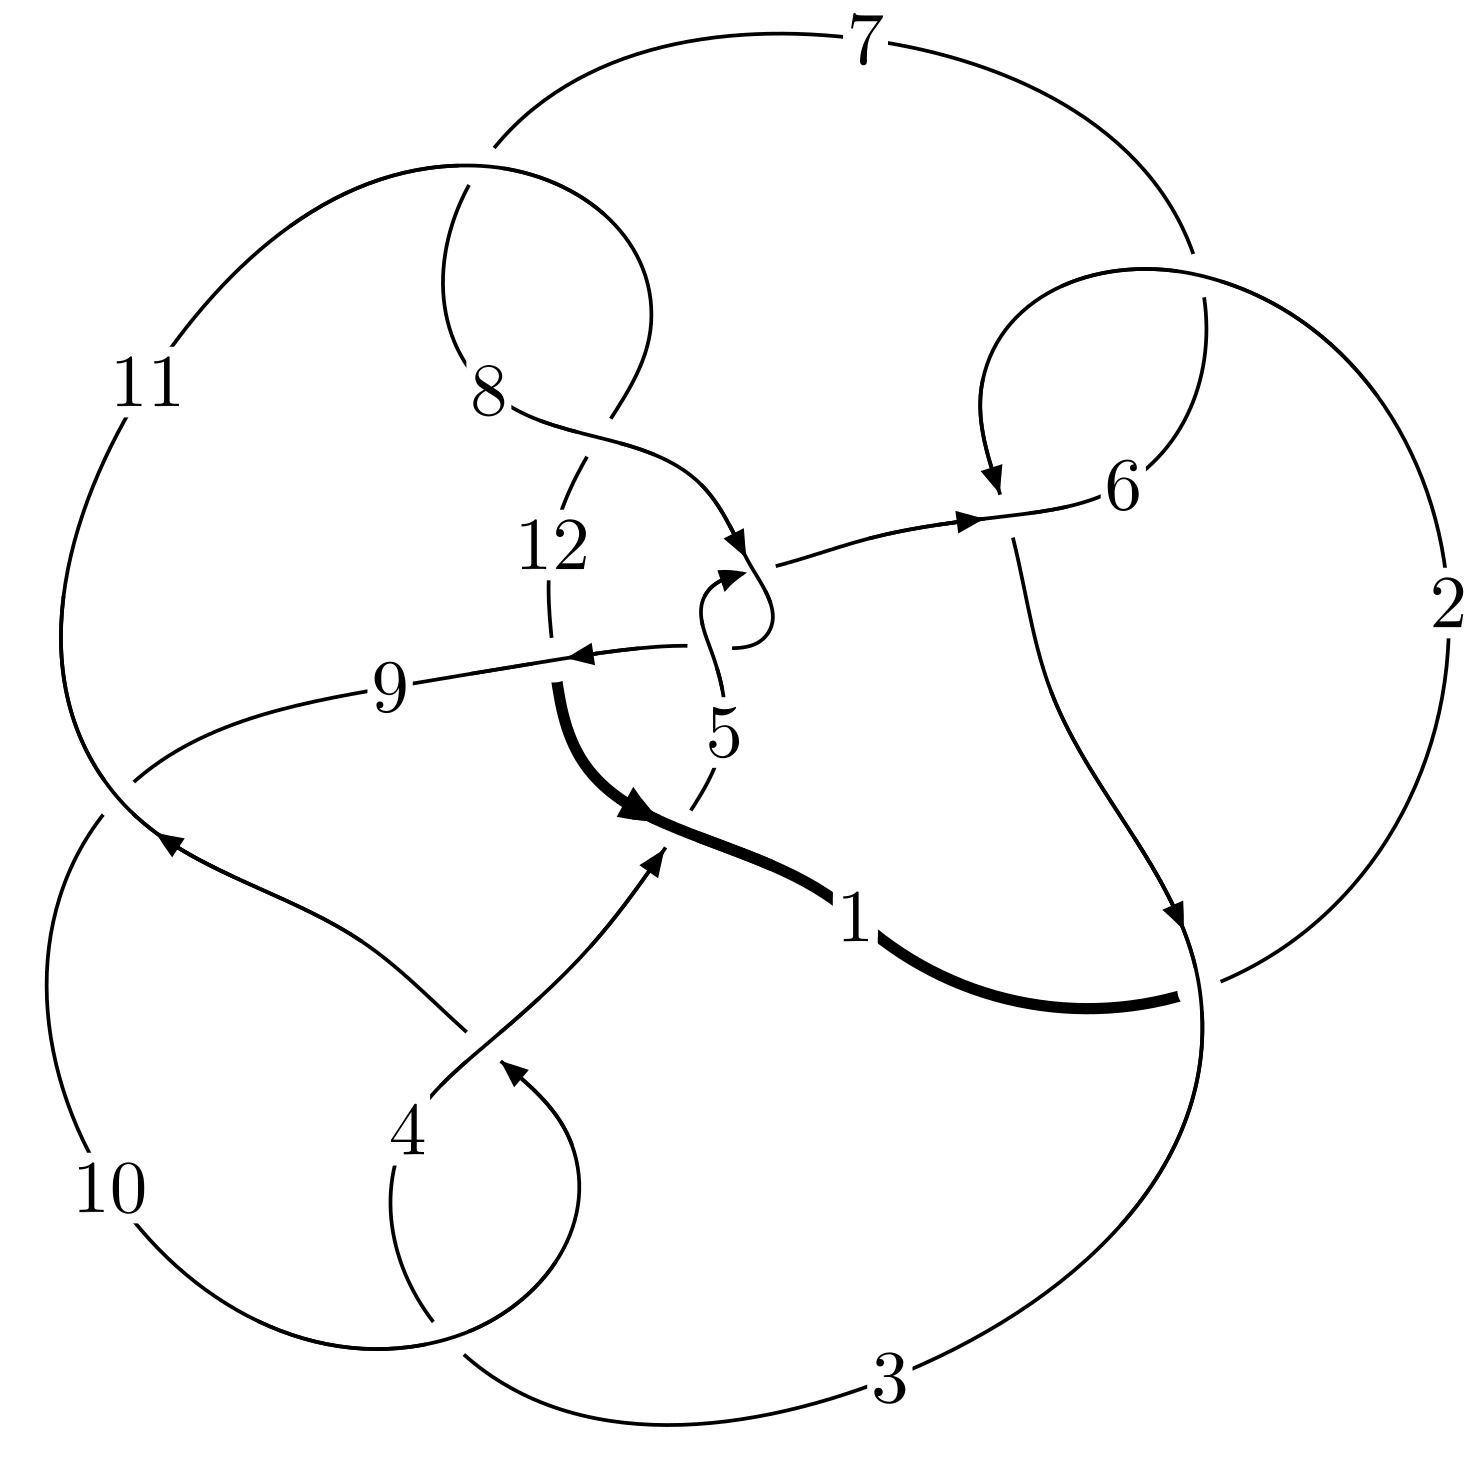
\includegraphics[width=112pt]{../../../GIT/diagram.site/Diagrams/png/2618_12n_0529.png}\\
\ \ \ A knot diagram\footnotemark}&
\allowdisplaybreaks
\textbf{Linearized knot diagam} \\
\cline{2-2}
 &
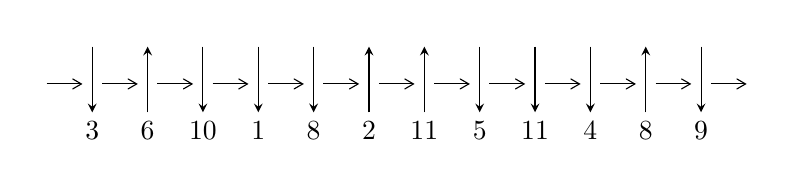
\begin{tikzpicture}[x=20pt, y=17pt]
	% nodes
	\node (C0) at (0, 0) {};
	\node (C1) at (1, 0) {};
	\node (C1U) at (1, +1) {};
	\node (C1D) at (1, -1) {3};

	\node (C2) at (2, 0) {};
	\node (C2U) at (2, +1) {};
	\node (C2D) at (2, -1) {6};

	\node (C3) at (3, 0) {};
	\node (C3U) at (3, +1) {};
	\node (C3D) at (3, -1) {10};

	\node (C4) at (4, 0) {};
	\node (C4U) at (4, +1) {};
	\node (C4D) at (4, -1) {1};

	\node (C5) at (5, 0) {};
	\node (C5U) at (5, +1) {};
	\node (C5D) at (5, -1) {8};

	\node (C6) at (6, 0) {};
	\node (C6U) at (6, +1) {};
	\node (C6D) at (6, -1) {2};

	\node (C7) at (7, 0) {};
	\node (C7U) at (7, +1) {};
	\node (C7D) at (7, -1) {11};

	\node (C8) at (8, 0) {};
	\node (C8U) at (8, +1) {};
	\node (C8D) at (8, -1) {5};

	\node (C9) at (9, 0) {};
	\node (C9U) at (9, +1) {};
	\node (C9D) at (9, -1) {11};

	\node (C10) at (10, 0) {};
	\node (C10U) at (10, +1) {};
	\node (C10D) at (10, -1) {4};

	\node (C11) at (11, 0) {};
	\node (C11U) at (11, +1) {};
	\node (C11D) at (11, -1) {8};

	\node (C12) at (12, 0) {};
	\node (C12U) at (12, +1) {};
	\node (C12D) at (12, -1) {9};
	\node (C13) at (13, 0) {};

	% arrows
	\draw[->,>={angle 60}]
	(C0) edge (C1) (C1) edge (C2) (C2) edge (C3) (C3) edge (C4) (C4) edge (C5) (C5) edge (C6) (C6) edge (C7) (C7) edge (C8) (C8) edge (C9) (C9) edge (C10) (C10) edge (C11) (C11) edge (C12) (C12) edge (C13) ;	\draw[->,>=stealth]
	(C1U) edge (C1D) (C2D) edge (C2U) (C3U) edge (C3D) (C4U) edge (C4D) (C5U) edge (C5D) (C6D) edge (C6U) (C7D) edge (C7U) (C8U) edge (C8D) (C9U) edge (C9D) (C10U) edge (C10D) (C11D) edge (C11U) (C12U) edge (C12D) ;
	\end{tikzpicture} \\
\hhline{~~} \\& 
\textbf{Solving Sequence} \\ \cline{2-2} 
 &
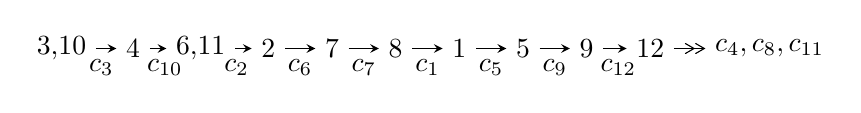
\begin{tikzpicture}[x=23pt, y=7pt]
	% node
	\node (A0) at (-1/8, 0) {3,10};
	\node (A1) at (1, 0) {4};
	\node (A2) at (33/16, 0) {6,11};
	\node (A3) at (25/8, 0) {2};
	\node (A4) at (33/8, 0) {7};
	\node (A5) at (41/8, 0) {8};
	\node (A6) at (49/8, 0) {1};
	\node (A7) at (57/8, 0) {5};
	\node (A8) at (65/8, 0) {9};
	\node (A9) at (73/8, 0) {12};
	\node (C1) at (1/2, -1) {$c_{3}$};
	\node (C2) at (3/2, -1) {$c_{10}$};
	\node (C3) at (21/8, -1) {$c_{2}$};
	\node (C4) at (29/8, -1) {$c_{6}$};
	\node (C5) at (37/8, -1) {$c_{7}$};
	\node (C6) at (45/8, -1) {$c_{1}$};
	\node (C7) at (53/8, -1) {$c_{5}$};
	\node (C8) at (61/8, -1) {$c_{9}$};
	\node (C9) at (69/8, -1) {$c_{12}$};
	\node (A10) at (11, 0) {$c_{4},c_{8},c_{11}$};

	% edge
	\draw[->,>=stealth]	
	(A0) edge (A1) (A1) edge (A2) (A2) edge (A3) (A3) edge (A4) (A4) edge (A5) (A5) edge (A6) (A6) edge (A7) (A7) edge (A8) (A8) edge (A9) ;
	\draw[->>,>={angle 60}]	
	(A9) edge (A10);
\end{tikzpicture} \\ 

\end{tabular} \\

\footnotetext{
The image of knot diagram is generated by the software ``\textbf{Draw programme}" developed by Andrew Bartholomew(\url{http://www.layer8.co.uk/maths/draw/index.htm\#Running-draw}), where we modified some parts for our purpose(\url{https://github.com/CATsTAILs/LinksPainter}).
}\phantom \\ \newline 
\centering \textbf{Ideals for irreducible components\footnotemark of $X_{\text{par}}$} 
 
\begin{align*}
I^u_{1}&=\langle 
8.62257\times10^{140} u^{80}-6.47276\times10^{140} u^{79}+\cdots+2.66122\times10^{142} b-8.68171\times10^{142},\\
\phantom{I^u_{1}}&\phantom{= \langle  }3.03432\times10^{143} u^{80}-2.26585\times10^{143} u^{79}+\cdots+6.25386\times10^{144} a-4.22144\times10^{145},\;u^{81}- u^{80}+\cdots+13 u+47\rangle \\
I^u_{2}&=\langle 
-5 u^{23}+u^{22}+\cdots+b-1,\;16 u^{23}-14 u^{22}+\cdots+a+33,\;u^{24}-7 u^{22}+\cdots+2 u+1\rangle \\
\\
\end{align*}
\raggedright * 2 irreducible components of $\dim_{\mathbb{C}}=0$, with total 105 representations.\\
\footnotetext{All coefficients of polynomials are rational numbers. But the coefficients are sometimes approximated in decimal forms when there is not enough margin.}
\newpage
\renewcommand{\arraystretch}{1}
\centering \section*{I. $I^u_{1}= \langle 8.62\times10^{140} u^{80}-6.47\times10^{140} u^{79}+\cdots+2.66\times10^{142} b-8.68\times10^{142},\;3.03\times10^{143} u^{80}-2.27\times10^{143} u^{79}+\cdots+6.25\times10^{144} a-4.22\times10^{145},\;u^{81}- u^{80}+\cdots+13 u+47 \rangle$}
\flushleft \textbf{(i) Arc colorings}\\
\begin{tabular}{m{7pt} m{180pt} m{7pt} m{180pt} }
\flushright $a_{3}=$&$\begin{pmatrix}1\\0\end{pmatrix}$ \\
\flushright $a_{10}=$&$\begin{pmatrix}0\\u\end{pmatrix}$ \\
\flushright $a_{4}=$&$\begin{pmatrix}1\\u^2\end{pmatrix}$ \\
\flushright $a_{6}=$&$\begin{pmatrix}-0.0485191 u^{80}+0.0362312 u^{79}+\cdots+15.1878 u+6.75014\\-0.0324008 u^{80}+0.0243225 u^{79}+\cdots+6.35687 u+3.26231\end{pmatrix}$ \\
\flushright $a_{11}=$&$\begin{pmatrix}- u\\- u^3+u\end{pmatrix}$ \\
\flushright $a_{2}=$&$\begin{pmatrix}0.145918 u^{80}-0.00189727 u^{79}+\cdots-15.4510 u-12.1681\\-0.0187396 u^{80}-0.0319668 u^{79}+\cdots-1.63055 u+2.79062\end{pmatrix}$ \\
\flushright $a_{7}=$&$\begin{pmatrix}0.0764253 u^{80}-0.0146344 u^{79}+\cdots-6.83981 u-7.33819\\0.0574398 u^{80}-0.0642603 u^{79}+\cdots-8.20882 u-3.09289\end{pmatrix}$ \\
\flushright $a_{8}=$&$\begin{pmatrix}0.169348 u^{80}-0.0360227 u^{79}+\cdots-13.2694 u-11.0124\\0.0617316 u^{80}-0.0482530 u^{79}+\cdots-7.07660 u-2.78079\end{pmatrix}$ \\
\flushright $a_{1}=$&$\begin{pmatrix}0.127178 u^{80}-0.0338641 u^{79}+\cdots-17.0815 u-9.37752\\-0.0187396 u^{80}-0.0319668 u^{79}+\cdots-1.63055 u+2.79062\end{pmatrix}$ \\
\flushright $a_{5}=$&$\begin{pmatrix}0.0973705 u^{80}+0.0318201 u^{79}+\cdots-1.32449 u-4.48371\\0.0209631 u^{80}+0.0149658 u^{79}+\cdots+2.54446 u-2.31091\end{pmatrix}$ \\
\flushright $a_{9}=$&$\begin{pmatrix}u^3\\u^5- u^3+u\end{pmatrix}$ \\
\flushright $a_{12}=$&$\begin{pmatrix}0.0533183 u^{80}-0.0156877 u^{79}+\cdots-12.0825 u-6.28809\\-0.0819438 u^{80}-0.00309381 u^{79}+\cdots+5.06453 u+6.74036\end{pmatrix}$\\&\end{tabular}
\flushleft \textbf{(ii) Obstruction class $= -1$}\\~\\
\flushleft \textbf{(iii) Cusp Shapes $= 0.574685 u^{80}-0.0343111 u^{79}+\cdots-42.1791 u-39.7887$}\\~\\
\newpage\renewcommand{\arraystretch}{1}
\flushleft \textbf{(iv) u-Polynomials at the component}\newline \\
\begin{tabular}{m{50pt}|m{274pt}}
Crossings & \hspace{64pt}u-Polynomials at each crossing \\
\hline $$\begin{aligned}c_{1}\end{aligned}$$&$\begin{aligned}
&u^{81}+47 u^{80}+\cdots-12 u-1
\end{aligned}$\\
\hline $$\begin{aligned}c_{2},c_{6}\end{aligned}$$&$\begin{aligned}
&u^{81}- u^{80}+\cdots+6 u^2+1
\end{aligned}$\\
\hline $$\begin{aligned}c_{3},c_{10}\end{aligned}$$&$\begin{aligned}
&u^{81}- u^{80}+\cdots+13 u+47
\end{aligned}$\\
\hline $$\begin{aligned}c_{4}\end{aligned}$$&$\begin{aligned}
&u^{81}-3 u^{80}+\cdots+1837 u+347
\end{aligned}$\\
\hline $$\begin{aligned}c_{5},c_{8}\end{aligned}$$&$\begin{aligned}
&u^{81}-3 u^{80}+\cdots-35 u-49
\end{aligned}$\\
\hline $$\begin{aligned}c_{7},c_{11}\end{aligned}$$&$\begin{aligned}
&u^{81}+5 u^{80}+\cdots-11394 u+9307
\end{aligned}$\\
\hline $$\begin{aligned}c_{9}\end{aligned}$$&$\begin{aligned}
&u^{81}+43 u^{80}+\cdots+30249 u+2209
\end{aligned}$\\
\hline $$\begin{aligned}c_{12}\end{aligned}$$&$\begin{aligned}
&u^{81}- u^{80}+\cdots-251686 u+41753
\end{aligned}$\\
\hline
\end{tabular}\\~\\
\newpage\renewcommand{\arraystretch}{1}
\flushleft \textbf{(v) Riley Polynomials at the component}\newline \\
\begin{tabular}{m{50pt}|m{274pt}}
Crossings & \hspace{64pt}Riley Polynomials at each crossing \\
\hline $$\begin{aligned}c_{1}\end{aligned}$$&$\begin{aligned}
&y^{81}-9 y^{80}+\cdots-28 y-1
\end{aligned}$\\
\hline $$\begin{aligned}c_{2},c_{6}\end{aligned}$$&$\begin{aligned}
&y^{81}+47 y^{80}+\cdots-12 y-1
\end{aligned}$\\
\hline $$\begin{aligned}c_{3},c_{10}\end{aligned}$$&$\begin{aligned}
&y^{81}-43 y^{80}+\cdots+30249 y-2209
\end{aligned}$\\
\hline $$\begin{aligned}c_{4}\end{aligned}$$&$\begin{aligned}
&y^{81}+37 y^{80}+\cdots-3637607 y-120409
\end{aligned}$\\
\hline $$\begin{aligned}c_{5},c_{8}\end{aligned}$$&$\begin{aligned}
&y^{81}+27 y^{80}+\cdots-50323 y-2401
\end{aligned}$\\
\hline $$\begin{aligned}c_{7},c_{11}\end{aligned}$$&$\begin{aligned}
&y^{81}+63 y^{80}+\cdots+678266132 y-86620249
\end{aligned}$\\
\hline $$\begin{aligned}c_{9}\end{aligned}$$&$\begin{aligned}
&y^{81}+5 y^{80}+\cdots-223295699 y-4879681
\end{aligned}$\\
\hline $$\begin{aligned}c_{12}\end{aligned}$$&$\begin{aligned}
&y^{81}-37 y^{80}+\cdots+94686312444 y-1743313009
\end{aligned}$\\
\hline
\end{tabular}\\~\\
\newpage\flushleft \textbf{(vi) Complex Volumes and Cusp Shapes}
$$\begin{array}{c|c|c}  
\text{Solutions to }I^u_{1}& \I (\text{vol} + \sqrt{-1}CS) & \text{Cusp shape}\\
 \hline 
\begin{aligned}
u &= \phantom{-}0.159420 + 0.995305 I \\
a &= \phantom{-}0.935421 + 0.685407 I \\
b &= -0.578486 - 1.135720 I\end{aligned}
 & -2.78412 + 4.09191 I & \phantom{-0.000000 } 0 \\ \hline\begin{aligned}
u &= \phantom{-}0.159420 - 0.995305 I \\
a &= \phantom{-}0.935421 - 0.685407 I \\
b &= -0.578486 + 1.135720 I\end{aligned}
 & -2.78412 - 4.09191 I & \phantom{-0.000000 } 0 \\ \hline\begin{aligned}
u &= \phantom{-}0.376854 + 0.905642 I \\
a &= -0.252327 + 0.170325 I \\
b &= \phantom{-}0.413913 - 0.717629 I\end{aligned}
 & \phantom{-}4.18971 - 1.89813 I & \phantom{-}6.48835 + 0. I\phantom{ +0.000000I} \\ \hline\begin{aligned}
u &= \phantom{-}0.376854 - 0.905642 I \\
a &= -0.252327 - 0.170325 I \\
b &= \phantom{-}0.413913 + 0.717629 I\end{aligned}
 & \phantom{-}4.18971 + 1.89813 I & \phantom{-}6.48835 + 0. I\phantom{ +0.000000I} \\ \hline\begin{aligned}
u &= -0.661263 + 0.704542 I \\
a &= \phantom{-}0.839577 - 0.272761 I \\
b &= -0.476366 + 1.005480 I\end{aligned}
 & \phantom{-}1.42827 - 2.25830 I & -4.00000 + 5.30334 I \\ \hline\begin{aligned}
u &= -0.661263 - 0.704542 I \\
a &= \phantom{-}0.839577 + 0.272761 I \\
b &= -0.476366 - 1.005480 I\end{aligned}
 & \phantom{-}1.42827 + 2.25830 I & -4.00000 - 5.30334 I \\ \hline\begin{aligned}
u &= -1.000680 + 0.339594 I \\
a &= -0.64504 + 1.66330 I \\
b &= \phantom{-}0.332392 + 1.158070 I\end{aligned}
 & \phantom{-}0.71275 + 3.59108 I & \phantom{-0.000000 } 0 \\ \hline\begin{aligned}
u &= -1.000680 - 0.339594 I \\
a &= -0.64504 - 1.66330 I \\
b &= \phantom{-}0.332392 - 1.158070 I\end{aligned}
 & \phantom{-}0.71275 - 3.59108 I & \phantom{-0.000000 } 0 \\ \hline\begin{aligned}
u &= -0.571724 + 0.894004 I \\
a &= -0.351532 + 0.151292 I \\
b &= \phantom{-}0.436363 - 0.928482 I\end{aligned}
 & \phantom{-}1.58675 + 1.13569 I & \phantom{-0.000000 } 0 \\ \hline\begin{aligned}
u &= -0.571724 - 0.894004 I \\
a &= -0.351532 - 0.151292 I \\
b &= \phantom{-}0.436363 + 0.928482 I\end{aligned}
 & \phantom{-}1.58675 - 1.13569 I & \phantom{-0.000000 } 0\\
 \hline 
 \end{array}$$\newpage$$\begin{array}{c|c|c}  
\text{Solutions to }I^u_{1}& \I (\text{vol} + \sqrt{-1}CS) & \text{Cusp shape}\\
 \hline 
\begin{aligned}
u &= -0.934622\phantom{ +0.000000I} \\
a &= -0.202474\phantom{ +0.000000I} \\
b &= \phantom{-}0.471310\phantom{ +0.000000I}\end{aligned}
 & -1.70013\phantom{ +0.000000I} & -4.55780\phantom{ +0.000000I} \\ \hline\begin{aligned}
u &= \phantom{-}0.883279 + 0.595878 I \\
a &= \phantom{-}0.630805 - 0.530733 I \\
b &= -0.525868 + 0.421987 I\end{aligned}
 & \phantom{-}3.21313 - 3.83074 I & \phantom{-0.000000 } 0 \\ \hline\begin{aligned}
u &= \phantom{-}0.883279 - 0.595878 I \\
a &= \phantom{-}0.630805 + 0.530733 I \\
b &= -0.525868 - 0.421987 I\end{aligned}
 & \phantom{-}3.21313 + 3.83074 I & \phantom{-0.000000 } 0 \\ \hline\begin{aligned}
u &= -0.408368 + 0.839079 I \\
a &= -1.46418 + 0.42247 I \\
b &= \phantom{-}0.924562 + 0.331227 I\end{aligned}
 & \phantom{-}0.85878 - 5.06052 I & \phantom{-0.000000 -}0. + 2.81038 I \\ \hline\begin{aligned}
u &= -0.408368 - 0.839079 I \\
a &= -1.46418 - 0.42247 I \\
b &= \phantom{-}0.924562 - 0.331227 I\end{aligned}
 & \phantom{-}0.85878 + 5.06052 I & \phantom{-0.000000 } 0. - 2.81038 I \\ \hline\begin{aligned}
u &= -0.979097 + 0.487895 I \\
a &= \phantom{-}0.105613 - 0.719977 I \\
b &= -0.931801 + 0.774121 I\end{aligned}
 & \phantom{-}3.71023 + 0.03758 I & \phantom{-0.000000 } 0 \\ \hline\begin{aligned}
u &= -0.979097 - 0.487895 I \\
a &= \phantom{-}0.105613 + 0.719977 I \\
b &= -0.931801 - 0.774121 I\end{aligned}
 & \phantom{-}3.71023 - 0.03758 I & \phantom{-0.000000 } 0 \\ \hline\begin{aligned}
u &= \phantom{-}0.322513 + 1.061320 I \\
a &= -0.810462 - 0.694013 I \\
b &= \phantom{-}0.599928 + 1.189190 I\end{aligned}
 & -1.78824 + 10.62680 I & \phantom{-0.000000 } 0 \\ \hline\begin{aligned}
u &= \phantom{-}0.322513 - 1.061320 I \\
a &= -0.810462 + 0.694013 I \\
b &= \phantom{-}0.599928 - 1.189190 I\end{aligned}
 & -1.78824 - 10.62680 I & \phantom{-0.000000 } 0 \\ \hline\begin{aligned}
u &= \phantom{-}0.823612 + 0.751253 I \\
a &= \phantom{-}0.811016 - 0.029992 I \\
b &= -0.409599 + 0.082280 I\end{aligned}
 & \phantom{-}3.40007 - 1.49524 I & \phantom{-0.000000 } 0\\
 \hline 
 \end{array}$$\newpage$$\begin{array}{c|c|c}  
\text{Solutions to }I^u_{1}& \I (\text{vol} + \sqrt{-1}CS) & \text{Cusp shape}\\
 \hline 
\begin{aligned}
u &= \phantom{-}0.823612 - 0.751253 I \\
a &= \phantom{-}0.811016 + 0.029992 I \\
b &= -0.409599 - 0.082280 I\end{aligned}
 & \phantom{-}3.40007 + 1.49524 I & \phantom{-0.000000 } 0 \\ \hline\begin{aligned}
u &= \phantom{-}0.864023 + 0.185989 I \\
a &= \phantom{-}1.90280 + 2.54662 I \\
b &= -0.066643 + 0.845765 I\end{aligned}
 & -2.91161 + 2.49317 I & -8.76964 - 0.67821 I \\ \hline\begin{aligned}
u &= \phantom{-}0.864023 - 0.185989 I \\
a &= \phantom{-}1.90280 - 2.54662 I \\
b &= -0.066643 - 0.845765 I\end{aligned}
 & -2.91161 - 2.49317 I & -8.76964 + 0.67821 I \\ \hline\begin{aligned}
u &= \phantom{-}1.100390 + 0.201043 I \\
a &= \phantom{-}1.00477 + 1.01305 I \\
b &= -0.740363 - 0.292523 I\end{aligned}
 & -4.23067 + 2.70934 I & \phantom{-0.000000 } 0 \\ \hline\begin{aligned}
u &= \phantom{-}1.100390 - 0.201043 I \\
a &= \phantom{-}1.00477 - 1.01305 I \\
b &= -0.740363 + 0.292523 I\end{aligned}
 & -4.23067 - 2.70934 I & \phantom{-0.000000 } 0 \\ \hline\begin{aligned}
u &= \phantom{-}0.871403 + 0.717699 I \\
a &= \phantom{-}0.976706 - 0.631023 I \\
b &= -0.042020 + 0.535241 I\end{aligned}
 & \phantom{-}3.36043 - 1.33032 I & \phantom{-0.000000 } 0 \\ \hline\begin{aligned}
u &= \phantom{-}0.871403 - 0.717699 I \\
a &= \phantom{-}0.976706 + 0.631023 I \\
b &= -0.042020 - 0.535241 I\end{aligned}
 & \phantom{-}3.36043 + 1.33032 I & \phantom{-0.000000 } 0 \\ \hline\begin{aligned}
u &= \phantom{-}1.122290 + 0.197548 I \\
a &= -1.04175 - 1.25015 I \\
b &= \phantom{-}0.313035 - 0.963622 I\end{aligned}
 & -4.22930 - 2.75874 I & \phantom{-0.000000 } 0 \\ \hline\begin{aligned}
u &= \phantom{-}1.122290 - 0.197548 I \\
a &= -1.04175 + 1.25015 I \\
b &= \phantom{-}0.313035 + 0.963622 I\end{aligned}
 & -4.22930 + 2.75874 I & \phantom{-0.000000 } 0 \\ \hline\begin{aligned}
u &= \phantom{-}1.081310 + 0.429427 I \\
a &= -0.239516 - 0.185534 I \\
b &= -0.32431 - 1.54232 I\end{aligned}
 & -7.39105 - 5.07513 I & \phantom{-0.000000 } 0\\
 \hline 
 \end{array}$$\newpage$$\begin{array}{c|c|c}  
\text{Solutions to }I^u_{1}& \I (\text{vol} + \sqrt{-1}CS) & \text{Cusp shape}\\
 \hline 
\begin{aligned}
u &= \phantom{-}1.081310 - 0.429427 I \\
a &= -0.239516 + 0.185534 I \\
b &= -0.32431 + 1.54232 I\end{aligned}
 & -7.39105 + 5.07513 I & \phantom{-0.000000 } 0 \\ \hline\begin{aligned}
u &= -0.353227 + 0.757360 I \\
a &= \phantom{-}1.13050 - 1.44697 I \\
b &= -0.309577 + 1.131200 I\end{aligned}
 & -4.70079 - 3.78323 I & -5.54818 + 3.30856 I \\ \hline\begin{aligned}
u &= -0.353227 - 0.757360 I \\
a &= \phantom{-}1.13050 + 1.44697 I \\
b &= -0.309577 - 1.131200 I\end{aligned}
 & -4.70079 + 3.78323 I & -5.54818 - 3.30856 I \\ \hline\begin{aligned}
u &= \phantom{-}1.116360 + 0.351305 I \\
a &= -1.05780 - 0.95057 I \\
b &= \phantom{-}0.666696 + 0.237202 I\end{aligned}
 & -4.33281 - 4.26606 I & \phantom{-0.000000 } 0 \\ \hline\begin{aligned}
u &= \phantom{-}1.116360 - 0.351305 I \\
a &= -1.05780 + 0.95057 I \\
b &= \phantom{-}0.666696 - 0.237202 I\end{aligned}
 & -4.33281 + 4.26606 I & \phantom{-0.000000 } 0 \\ \hline\begin{aligned}
u &= \phantom{-}1.097800 + 0.427856 I \\
a &= \phantom{-}1.57748 + 0.94414 I \\
b &= -0.811505 + 1.002040 I\end{aligned}
 & \phantom{-}2.99739 - 6.42104 I & \phantom{-0.000000 } 0 \\ \hline\begin{aligned}
u &= \phantom{-}1.097800 - 0.427856 I \\
a &= \phantom{-}1.57748 - 0.94414 I \\
b &= -0.811505 - 1.002040 I\end{aligned}
 & \phantom{-}2.99739 + 6.42104 I & \phantom{-0.000000 } 0 \\ \hline\begin{aligned}
u &= \phantom{-}0.922762 + 0.740121 I \\
a &= -0.415168 - 0.652065 I \\
b &= \phantom{-}0.271496 + 0.211929 I\end{aligned}
 & \phantom{-}3.08566 - 4.17180 I & \phantom{-0.000000 } 0 \\ \hline\begin{aligned}
u &= \phantom{-}0.922762 - 0.740121 I \\
a &= -0.415168 + 0.652065 I \\
b &= \phantom{-}0.271496 - 0.211929 I\end{aligned}
 & \phantom{-}3.08566 + 4.17180 I & \phantom{-0.000000 } 0 \\ \hline\begin{aligned}
u &= -0.991780 + 0.652953 I \\
a &= -1.84179 + 0.76782 I \\
b &= \phantom{-}0.394401 + 1.134090 I\end{aligned}
 & \phantom{-}0.43873 + 7.49699 I & \phantom{-0.000000 } 0\\
 \hline 
 \end{array}$$\newpage$$\begin{array}{c|c|c}  
\text{Solutions to }I^u_{1}& \I (\text{vol} + \sqrt{-1}CS) & \text{Cusp shape}\\
 \hline 
\begin{aligned}
u &= -0.991780 - 0.652953 I \\
a &= -1.84179 - 0.76782 I \\
b &= \phantom{-}0.394401 - 1.134090 I\end{aligned}
 & \phantom{-}0.43873 - 7.49699 I & \phantom{-0.000000 } 0 \\ \hline\begin{aligned}
u &= \phantom{-}1.162730 + 0.284953 I \\
a &= -0.009432 + 0.485623 I \\
b &= \phantom{-}0.27944 + 1.42871 I\end{aligned}
 & -9.09751 + 0.85503 I & \phantom{-0.000000 } 0 \\ \hline\begin{aligned}
u &= \phantom{-}1.162730 - 0.284953 I \\
a &= -0.009432 - 0.485623 I \\
b &= \phantom{-}0.27944 - 1.42871 I\end{aligned}
 & -9.09751 - 0.85503 I & \phantom{-0.000000 } 0 \\ \hline\begin{aligned}
u &= -0.743234 + 0.302673 I \\
a &= \phantom{-}1.265020 + 0.224679 I \\
b &= -0.598633 + 1.007620 I\end{aligned}
 & \phantom{-}1.64504 - 0.79136 I & -7.66851 - 3.15531 I \\ \hline\begin{aligned}
u &= -0.743234 - 0.302673 I \\
a &= \phantom{-}1.265020 - 0.224679 I \\
b &= -0.598633 - 1.007620 I\end{aligned}
 & \phantom{-}1.64504 + 0.79136 I & -7.66851 + 3.15531 I \\ \hline\begin{aligned}
u &= -1.118710 + 0.488890 I \\
a &= \phantom{-}1.89475 - 0.05980 I \\
b &= -0.542651 - 1.179660 I\end{aligned}
 & -6.90163 + 2.26075 I & \phantom{-0.000000 } 0 \\ \hline\begin{aligned}
u &= -1.118710 - 0.488890 I \\
a &= \phantom{-}1.89475 + 0.05980 I \\
b &= -0.542651 + 1.179660 I\end{aligned}
 & -6.90163 - 2.26075 I & \phantom{-0.000000 } 0 \\ \hline\begin{aligned}
u &= -1.145040 + 0.505621 I \\
a &= -0.597188 + 0.555247 I \\
b &= \phantom{-}1.028760 - 0.304158 I\end{aligned}
 & -3.26600 + 3.64539 I & \phantom{-0.000000 } 0 \\ \hline\begin{aligned}
u &= -1.145040 - 0.505621 I \\
a &= -0.597188 - 0.555247 I \\
b &= \phantom{-}1.028760 + 0.304158 I\end{aligned}
 & -3.26600 - 3.64539 I & \phantom{-0.000000 } 0 \\ \hline\begin{aligned}
u &= -0.183670 + 0.715881 I \\
a &= \phantom{-}1.45549 - 0.28504 I \\
b &= -0.716431 - 0.354969 I\end{aligned}
 & -0.514533 + 0.940856 I & -1.24894 - 2.13001 I\\
 \hline 
 \end{array}$$\newpage$$\begin{array}{c|c|c}  
\text{Solutions to }I^u_{1}& \I (\text{vol} + \sqrt{-1}CS) & \text{Cusp shape}\\
 \hline 
\begin{aligned}
u &= -0.183670 - 0.715881 I \\
a &= \phantom{-}1.45549 + 0.28504 I \\
b &= -0.716431 + 0.354969 I\end{aligned}
 & -0.514533 - 0.940856 I & -1.24894 + 2.13001 I \\ \hline\begin{aligned}
u &= -1.139740 + 0.579388 I \\
a &= -1.94101 + 0.08618 I \\
b &= \phantom{-}0.512467 + 1.158430 I\end{aligned}
 & -7.02831 + 8.88570 I & \phantom{-0.000000 } 0 \\ \hline\begin{aligned}
u &= -1.139740 - 0.579388 I \\
a &= -1.94101 - 0.08618 I \\
b &= \phantom{-}0.512467 - 1.158430 I\end{aligned}
 & -7.02831 - 8.88570 I & \phantom{-0.000000 } 0 \\ \hline\begin{aligned}
u &= -0.634187 + 0.341977 I \\
a &= -1.90217 + 0.43344 I \\
b &= \phantom{-}0.915109 + 0.975916 I\end{aligned}
 & \phantom{-}4.92844 + 3.68094 I & -2.52917 - 1.30807 I \\ \hline\begin{aligned}
u &= -0.634187 - 0.341977 I \\
a &= -1.90217 - 0.43344 I \\
b &= \phantom{-}0.915109 - 0.975916 I\end{aligned}
 & \phantom{-}4.92844 - 3.68094 I & -2.52917 + 1.30807 I \\ \hline\begin{aligned}
u &= -1.136150 + 0.610179 I \\
a &= \phantom{-}0.747989 - 0.641986 I \\
b &= -1.136880 + 0.243931 I\end{aligned}
 & -1.34866 + 10.46180 I & \phantom{-0.000000 } 0 \\ \hline\begin{aligned}
u &= -1.136150 - 0.610179 I \\
a &= \phantom{-}0.747989 + 0.641986 I \\
b &= -1.136880 - 0.243931 I\end{aligned}
 & -1.34866 - 10.46180 I & \phantom{-0.000000 } 0 \\ \hline\begin{aligned}
u &= -1.070200 + 0.734551 I \\
a &= \phantom{-}1.296960 - 0.360784 I \\
b &= -0.378710 - 1.178060 I\end{aligned}
 & \phantom{-}0.09459 + 4.85619 I & \phantom{-0.000000 } 0 \\ \hline\begin{aligned}
u &= -1.070200 - 0.734551 I \\
a &= \phantom{-}1.296960 + 0.360784 I \\
b &= -0.378710 + 1.178060 I\end{aligned}
 & \phantom{-}0.09459 - 4.85619 I & \phantom{-0.000000 } 0 \\ \hline\begin{aligned}
u &= \phantom{-}0.637063 + 0.218185 I \\
a &= -1.32663 - 1.92334 I \\
b &= \phantom{-}0.03800 - 1.49521 I\end{aligned}
 & -5.48699 + 1.94976 I & \phantom{-}2.72009 + 1.05128 I\\
 \hline 
 \end{array}$$\newpage$$\begin{array}{c|c|c}  
\text{Solutions to }I^u_{1}& \I (\text{vol} + \sqrt{-1}CS) & \text{Cusp shape}\\
 \hline 
\begin{aligned}
u &= \phantom{-}0.637063 - 0.218185 I \\
a &= -1.32663 + 1.92334 I \\
b &= \phantom{-}0.03800 + 1.49521 I\end{aligned}
 & -5.48699 - 1.94976 I & \phantom{-}2.72009 - 1.05128 I \\ \hline\begin{aligned}
u &= -0.311386 + 0.591390 I \\
a &= -0.80934 + 2.32791 I \\
b &= \phantom{-}0.226255 - 1.139810 I\end{aligned}
 & -4.49439 + 2.07707 I & -5.39720 - 3.30118 I \\ \hline\begin{aligned}
u &= -0.311386 - 0.591390 I \\
a &= -0.80934 - 2.32791 I \\
b &= \phantom{-}0.226255 + 1.139810 I\end{aligned}
 & -4.49439 - 2.07707 I & -5.39720 + 3.30118 I \\ \hline\begin{aligned}
u &= \phantom{-}0.985820 + 0.912507 I \\
a &= -0.636717 + 0.039730 I \\
b &= \phantom{-}0.201679 - 0.628086 I\end{aligned}
 & \phantom{-}2.79450 - 4.44773 I & \phantom{-0.000000 } 0 \\ \hline\begin{aligned}
u &= \phantom{-}0.985820 - 0.912507 I \\
a &= -0.636717 - 0.039730 I \\
b &= \phantom{-}0.201679 + 0.628086 I\end{aligned}
 & \phantom{-}2.79450 + 4.44773 I & \phantom{-0.000000 } 0 \\ \hline\begin{aligned}
u &= \phantom{-}1.359520 + 0.164573 I \\
a &= -0.399737 - 1.222220 I \\
b &= \phantom{-}0.068318 - 0.573572 I\end{aligned}
 & -4.98357 - 3.68959 I & \phantom{-0.000000 } 0 \\ \hline\begin{aligned}
u &= \phantom{-}1.359520 - 0.164573 I \\
a &= -0.399737 + 1.222220 I \\
b &= \phantom{-}0.068318 + 0.573572 I\end{aligned}
 & -4.98357 + 3.68959 I & \phantom{-0.000000 } 0 \\ \hline\begin{aligned}
u &= \phantom{-}1.258050 + 0.575219 I \\
a &= -1.49315 - 0.54735 I \\
b &= \phantom{-}0.651128 - 1.243060 I\end{aligned}
 & -6.14816 - 9.70514 I & \phantom{-0.000000 } 0 \\ \hline\begin{aligned}
u &= \phantom{-}1.258050 - 0.575219 I \\
a &= -1.49315 + 0.54735 I \\
b &= \phantom{-}0.651128 + 1.243060 I\end{aligned}
 & -6.14816 + 9.70514 I & \phantom{-0.000000 } 0 \\ \hline\begin{aligned}
u &= -1.290740 + 0.507998 I \\
a &= \phantom{-}0.736660 - 0.702992 I \\
b &= -0.356631 - 1.170940 I\end{aligned}
 & -0.49084 + 6.69889 I & \phantom{-0.000000 } 0\\
 \hline 
 \end{array}$$\newpage$$\begin{array}{c|c|c}  
\text{Solutions to }I^u_{1}& \I (\text{vol} + \sqrt{-1}CS) & \text{Cusp shape}\\
 \hline 
\begin{aligned}
u &= -1.290740 - 0.507998 I \\
a &= \phantom{-}0.736660 + 0.702992 I \\
b &= -0.356631 + 1.170940 I\end{aligned}
 & -0.49084 - 6.69889 I & \phantom{-0.000000 } 0 \\ \hline\begin{aligned}
u &= \phantom{-}1.240140 + 0.660502 I \\
a &= \phantom{-}1.56088 + 0.45637 I \\
b &= -0.65000 + 1.29438 I\end{aligned}
 & -4.6334 - 16.7910 I & \phantom{-0.000000 } 0 \\ \hline\begin{aligned}
u &= \phantom{-}1.240140 - 0.660502 I \\
a &= \phantom{-}1.56088 - 0.45637 I \\
b &= -0.65000 - 1.29438 I\end{aligned}
 & -4.6334 + 16.7910 I & \phantom{-0.000000 } 0 \\ \hline\begin{aligned}
u &= -1.38465 + 0.37974 I \\
a &= \phantom{-}0.139313 - 0.158138 I \\
b &= \phantom{-}0.414696 - 1.149390 I\end{aligned}
 & -7.77183 + 0.76959 I & \phantom{-0.000000 } 0 \\ \hline\begin{aligned}
u &= -1.38465 - 0.37974 I \\
a &= \phantom{-}0.139313 + 0.158138 I \\
b &= \phantom{-}0.414696 + 1.149390 I\end{aligned}
 & -7.77183 - 0.76959 I & \phantom{-0.000000 } 0 \\ \hline\begin{aligned}
u &= \phantom{-}0.417926 + 0.357171 I \\
a &= -0.87838 - 1.58477 I \\
b &= \phantom{-}0.857230 + 0.892954 I\end{aligned}
 & \phantom{-}5.13693 + 2.84021 I & \phantom{-}1.05922 - 6.16779 I \\ \hline\begin{aligned}
u &= \phantom{-}0.417926 - 0.357171 I \\
a &= -0.87838 + 1.58477 I \\
b &= \phantom{-}0.857230 - 0.892954 I\end{aligned}
 & \phantom{-}5.13693 - 2.84021 I & \phantom{-}1.05922 + 6.16779 I \\ \hline\begin{aligned}
u &= -1.47404 + 0.21229 I \\
a &= -0.048590 + 0.308635 I \\
b &= -0.384894 + 1.161020 I\end{aligned}
 & -8.06565 - 6.08851 I & \phantom{-0.000000 } 0 \\ \hline\begin{aligned}
u &= -1.47404 - 0.21229 I \\
a &= -0.048590 - 0.308635 I \\
b &= -0.384894 - 1.161020 I\end{aligned}
 & -8.06565 + 6.08851 I & \phantom{-0.000000 } 0 \\ \hline\begin{aligned}
u &= -0.238068 + 0.402940 I \\
a &= \phantom{-}1.102460 - 0.088285 I \\
b &= -0.300155 - 0.543538 I\end{aligned}
 & -0.171294 + 1.043260 I & -3.00612 - 6.15581 I\\
 \hline 
 \end{array}$$\newpage$$\begin{array}{c|c|c}  
\text{Solutions to }I^u_{1}& \I (\text{vol} + \sqrt{-1}CS) & \text{Cusp shape}\\
 \hline 
\begin{aligned}
u &= -0.238068 - 0.402940 I \\
a &= \phantom{-}1.102460 + 0.088285 I \\
b &= -0.300155 + 0.543538 I\end{aligned}
 & -0.171294 - 1.043260 I & -3.00612 + 6.15581 I\\
 \hline 
 \end{array}$$\newpage\newpage\renewcommand{\arraystretch}{1}
\centering \section*{II. $I^u_{2}= \langle -5 u^{23}+u^{22}+\cdots+b-1,\;16 u^{23}-14 u^{22}+\cdots+a+33,\;u^{24}-7 u^{22}+\cdots+2 u+1 \rangle$}
\flushleft \textbf{(i) Arc colorings}\\
\begin{tabular}{m{7pt} m{180pt} m{7pt} m{180pt} }
\flushright $a_{3}=$&$\begin{pmatrix}1\\0\end{pmatrix}$ \\
\flushright $a_{10}=$&$\begin{pmatrix}0\\u\end{pmatrix}$ \\
\flushright $a_{4}=$&$\begin{pmatrix}1\\u^2\end{pmatrix}$ \\
\flushright $a_{6}=$&$\begin{pmatrix}-16 u^{23}+14 u^{22}+\cdots-24 u-33\\5 u^{23}- u^{22}+\cdots-7 u+1\end{pmatrix}$ \\
\flushright $a_{11}=$&$\begin{pmatrix}- u\\- u^3+u\end{pmatrix}$ \\
\flushright $a_{2}=$&$\begin{pmatrix}8 u^{23}- u^{22}+\cdots-16 u+10\\u^{23}-7 u^{21}+\cdots-2 u-1\end{pmatrix}$ \\
\flushright $a_{7}=$&$\begin{pmatrix}-15 u^{23}+6 u^{22}+\cdots-4 u-20\\3 u^{23}-4 u^{22}+\cdots+13 u+8\end{pmatrix}$ \\
\flushright $a_{8}=$&$\begin{pmatrix}-18 u^{23}+6 u^{22}+\cdots+u-21\\4 u^{23}-4 u^{22}+\cdots+11 u+9\end{pmatrix}$ \\
\flushright $a_{1}=$&$\begin{pmatrix}9 u^{23}- u^{22}+\cdots-18 u+9\\u^{23}-7 u^{21}+\cdots-2 u-1\end{pmatrix}$ \\
\flushright $a_{5}=$&$\begin{pmatrix}-8 u^{23}+7 u^{22}+\cdots-18 u-26\\u^{23}+u^{22}+\cdots-5 u+1\end{pmatrix}$ \\
\flushright $a_{9}=$&$\begin{pmatrix}u^3\\u^5- u^3+u\end{pmatrix}$ \\
\flushright $a_{12}=$&$\begin{pmatrix}8 u^{23}- u^{22}+\cdots-16 u+9\\- u^{19}+6 u^{17}+\cdots+2 u-2\end{pmatrix}$\\&\end{tabular}
\flushleft \textbf{(ii) Obstruction class $= 1$}\\~\\
\flushleft \textbf{(iii) Cusp Shapes $= 25 u^{23}-22 u^{22}-171 u^{21}+195 u^{20}+576 u^{19}-827 u^{18}-1216 u^{17}+2202 u^{16}+1672 u^{15}-4057 u^{14}-1435 u^{13}+5422 u^{12}+575 u^{11}-5408 u^{10}+259 u^9+4100 u^8-511 u^7-2403 u^6+358 u^5+1038 u^4-121 u^3-324 u^2+10 u+45$}\\~\\
\newpage\renewcommand{\arraystretch}{1}
\flushleft \textbf{(iv) u-Polynomials at the component}\newline \\
\begin{tabular}{m{50pt}|m{274pt}}
Crossings & \hspace{64pt}u-Polynomials at each crossing \\
\hline $$\begin{aligned}c_{1}\end{aligned}$$&$\begin{aligned}
&u^{24}-16 u^{23}+\cdots-21 u+1
\end{aligned}$\\
\hline $$\begin{aligned}c_{2}\end{aligned}$$&$\begin{aligned}
&u^{24}+8 u^{22}+\cdots+u+1
\end{aligned}$\\
\hline $$\begin{aligned}c_{3}\end{aligned}$$&$\begin{aligned}
&u^{24}-7 u^{22}+\cdots+2 u+1
\end{aligned}$\\
\hline $$\begin{aligned}c_{4}\end{aligned}$$&$\begin{aligned}
&u^{24}+2 u^{23}+\cdots-2 u^2+1
\end{aligned}$\\
\hline $$\begin{aligned}c_{5}\end{aligned}$$&$\begin{aligned}
&u^{24}-4 u^{23}+\cdots-4 u+1
\end{aligned}$\\
\hline $$\begin{aligned}c_{6}\end{aligned}$$&$\begin{aligned}
&u^{24}+8 u^{22}+\cdots- u+1
\end{aligned}$\\
\hline $$\begin{aligned}c_{7}\end{aligned}$$&$\begin{aligned}
&u^{24}+2 u^{22}+\cdots+u+1
\end{aligned}$\\
\hline $$\begin{aligned}c_{8}\end{aligned}$$&$\begin{aligned}
&u^{24}+4 u^{23}+\cdots+4 u+1
\end{aligned}$\\
\hline $$\begin{aligned}c_{9}\end{aligned}$$&$\begin{aligned}
&u^{24}-14 u^{23}+\cdots-16 u+1
\end{aligned}$\\
\hline $$\begin{aligned}c_{10}\end{aligned}$$&$\begin{aligned}
&u^{24}-7 u^{22}+\cdots-2 u+1
\end{aligned}$\\
\hline $$\begin{aligned}c_{11}\end{aligned}$$&$\begin{aligned}
&u^{24}+2 u^{22}+\cdots- u+1
\end{aligned}$\\
\hline $$\begin{aligned}c_{12}\end{aligned}$$&$\begin{aligned}
&u^{24}+8 u^{23}+\cdots-203 u+103
\end{aligned}$\\
\hline
\end{tabular}\\~\\
\newpage\renewcommand{\arraystretch}{1}
\flushleft \textbf{(v) Riley Polynomials at the component}\newline \\
\begin{tabular}{m{50pt}|m{274pt}}
Crossings & \hspace{64pt}Riley Polynomials at each crossing \\
\hline $$\begin{aligned}c_{1}\end{aligned}$$&$\begin{aligned}
&y^{24}-32 y^{22}+\cdots-23 y+1
\end{aligned}$\\
\hline $$\begin{aligned}c_{2},c_{6}\end{aligned}$$&$\begin{aligned}
&y^{24}+16 y^{23}+\cdots+21 y+1
\end{aligned}$\\
\hline $$\begin{aligned}c_{3},c_{10}\end{aligned}$$&$\begin{aligned}
&y^{24}-14 y^{23}+\cdots-16 y+1
\end{aligned}$\\
\hline $$\begin{aligned}c_{4}\end{aligned}$$&$\begin{aligned}
&y^{24}+18 y^{23}+\cdots-4 y+1
\end{aligned}$\\
\hline $$\begin{aligned}c_{5},c_{8}\end{aligned}$$&$\begin{aligned}
&y^{24}+16 y^{23}+\cdots+20 y+1
\end{aligned}$\\
\hline $$\begin{aligned}c_{7},c_{11}\end{aligned}$$&$\begin{aligned}
&y^{24}+4 y^{23}+\cdots-11 y+1
\end{aligned}$\\
\hline $$\begin{aligned}c_{9}\end{aligned}$$&$\begin{aligned}
&y^{24}+6 y^{23}+\cdots-8 y+1
\end{aligned}$\\
\hline $$\begin{aligned}c_{12}\end{aligned}$$&$\begin{aligned}
&y^{24}-8 y^{23}+\cdots+12145 y+10609
\end{aligned}$\\
\hline
\end{tabular}\\~\\
\newpage\flushleft \textbf{(vi) Complex Volumes and Cusp Shapes}
$$\begin{array}{c|c|c}  
\text{Solutions to }I^u_{2}& \I (\text{vol} + \sqrt{-1}CS) & \text{Cusp shape}\\
 \hline 
\begin{aligned}
u &= \phantom{-}0.760804 + 0.607035 I \\
a &= -1.49179 + 0.04895 I \\
b &= \phantom{-}0.887524 - 0.776961 I\end{aligned}
 & \phantom{-}5.70049 - 4.53187 I & \phantom{-}3.10527 + 6.80987 I \\ \hline\begin{aligned}
u &= \phantom{-}0.760804 - 0.607035 I \\
a &= -1.49179 - 0.04895 I \\
b &= \phantom{-}0.887524 + 0.776961 I\end{aligned}
 & \phantom{-}5.70049 + 4.53187 I & \phantom{-}3.10527 - 6.80987 I \\ \hline\begin{aligned}
u &= \phantom{-}0.692071 + 0.781521 I \\
a &= \phantom{-}0.611885 - 0.793457 I \\
b &= -0.339703 + 0.732138 I\end{aligned}
 & \phantom{-}3.33432 - 2.30280 I & -2.18873 + 5.34734 I \\ \hline\begin{aligned}
u &= \phantom{-}0.692071 - 0.781521 I \\
a &= \phantom{-}0.611885 + 0.793457 I \\
b &= -0.339703 - 0.732138 I\end{aligned}
 & \phantom{-}3.33432 + 2.30280 I & -2.18873 - 5.34734 I \\ \hline\begin{aligned}
u &= -0.716982 + 0.459544 I \\
a &= -0.680089 + 0.749202 I \\
b &= \phantom{-}0.874697 - 1.033040 I\end{aligned}
 & \phantom{-}4.95705 - 1.97528 I & -0.77501 - 2.33256 I \\ \hline\begin{aligned}
u &= -0.716982 - 0.459544 I \\
a &= -0.680089 - 0.749202 I \\
b &= \phantom{-}0.874697 + 1.033040 I\end{aligned}
 & \phantom{-}4.95705 + 1.97528 I & -0.77501 + 2.33256 I \\ \hline\begin{aligned}
u &= -1.044620 + 0.486468 I \\
a &= \phantom{-}1.50313 - 1.01455 I \\
b &= -0.707939 - 1.076430 I\end{aligned}
 & \phantom{-}3.79667 + 5.88099 I & \phantom{-}0.70835 - 4.51294 I \\ \hline\begin{aligned}
u &= -1.044620 - 0.486468 I \\
a &= \phantom{-}1.50313 + 1.01455 I \\
b &= -0.707939 + 1.076430 I\end{aligned}
 & \phantom{-}3.79667 - 5.88099 I & \phantom{-}0.70835 + 4.51294 I \\ \hline\begin{aligned}
u &= \phantom{-}0.982224 + 0.632402 I \\
a &= \phantom{-}0.066377 + 0.727471 I \\
b &= -0.725173 - 0.698599 I\end{aligned}
 & \phantom{-}4.98117 - 0.35208 I & \phantom{-}2.23151 + 0.17854 I \\ \hline\begin{aligned}
u &= \phantom{-}0.982224 - 0.632402 I \\
a &= \phantom{-}0.066377 - 0.727471 I \\
b &= -0.725173 + 0.698599 I\end{aligned}
 & \phantom{-}4.98117 + 0.35208 I & \phantom{-}2.23151 - 0.17854 I\\
 \hline 
 \end{array}$$\newpage$$\begin{array}{c|c|c}  
\text{Solutions to }I^u_{2}& \I (\text{vol} + \sqrt{-1}CS) & \text{Cusp shape}\\
 \hline 
\begin{aligned}
u &= \phantom{-}1.210080 + 0.127545 I \\
a &= \phantom{-}0.196543 + 0.090225 I \\
b &= \phantom{-}0.070686 + 1.309280 I\end{aligned}
 & -7.87423 - 3.04176 I & -7.80879 + 2.61074 I \\ \hline\begin{aligned}
u &= \phantom{-}1.210080 - 0.127545 I \\
a &= \phantom{-}0.196543 - 0.090225 I \\
b &= \phantom{-}0.070686 - 1.309280 I\end{aligned}
 & -7.87423 + 3.04176 I & -7.80879 - 2.61074 I \\ \hline\begin{aligned}
u &= -0.568852 + 0.486026 I \\
a &= \phantom{-}0.778900 + 0.647406 I \\
b &= -0.474721 + 1.003620 I\end{aligned}
 & \phantom{-}2.29472 - 1.15093 I & \phantom{-}2.64163 + 1.71093 I \\ \hline\begin{aligned}
u &= -0.568852 - 0.486026 I \\
a &= \phantom{-}0.778900 - 0.647406 I \\
b &= -0.474721 - 1.003620 I\end{aligned}
 & \phantom{-}2.29472 + 1.15093 I & \phantom{-}2.64163 - 1.71093 I \\ \hline\begin{aligned}
u &= \phantom{-}0.732837 + 0.096465 I \\
a &= \phantom{-}1.22326 + 2.46457 I \\
b &= -0.04279 + 1.41632 I\end{aligned}
 & -5.93011 + 2.08072 I & -15.0441 - 4.1088 I \\ \hline\begin{aligned}
u &= \phantom{-}0.732837 - 0.096465 I \\
a &= \phantom{-}1.22326 - 2.46457 I \\
b &= -0.04279 - 1.41632 I\end{aligned}
 & -5.93011 - 2.08072 I & -15.0441 + 4.1088 I \\ \hline\begin{aligned}
u &= \phantom{-}0.970626 + 0.826369 I \\
a &= \phantom{-}0.040532 - 0.461280 I \\
b &= \phantom{-}0.152881 + 0.624525 I\end{aligned}
 & \phantom{-}2.52482 - 3.79144 I & -6.34052 - 1.00053 I \\ \hline\begin{aligned}
u &= \phantom{-}0.970626 - 0.826369 I \\
a &= \phantom{-}0.040532 + 0.461280 I \\
b &= \phantom{-}0.152881 - 0.624525 I\end{aligned}
 & \phantom{-}2.52482 + 3.79144 I & -6.34052 + 1.00053 I \\ \hline\begin{aligned}
u &= -1.133250 + 0.654883 I \\
a &= -1.105590 + 0.663064 I \\
b &= \phantom{-}0.306177 + 1.173280 I\end{aligned}
 & \phantom{-}0.26786 + 5.91058 I & -1.36806 - 6.09267 I \\ \hline\begin{aligned}
u &= -1.133250 - 0.654883 I \\
a &= -1.105590 - 0.663064 I \\
b &= \phantom{-}0.306177 - 1.173280 I\end{aligned}
 & \phantom{-}0.26786 - 5.91058 I & -1.36806 + 6.09267 I\\
 \hline 
 \end{array}$$\newpage$$\begin{array}{c|c|c}  
\text{Solutions to }I^u_{2}& \I (\text{vol} + \sqrt{-1}CS) & \text{Cusp shape}\\
 \hline 
\begin{aligned}
u &= -1.310450 + 0.138714 I \\
a &= -0.42360 + 1.66109 I \\
b &= \phantom{-}0.128205 + 0.671742 I\end{aligned}
 & -5.27306 + 3.87856 I & -18.3514 - 11.3041 I \\ \hline\begin{aligned}
u &= -1.310450 - 0.138714 I \\
a &= -0.42360 - 1.66109 I \\
b &= \phantom{-}0.128205 - 0.671742 I\end{aligned}
 & -5.27306 - 3.87856 I & -18.3514 + 11.3041 I \\ \hline\begin{aligned}
u &= -0.574501 + 0.081525 I \\
a &= \phantom{-}1.78044 - 3.44622 I \\
b &= -0.129839 + 0.528164 I\end{aligned}
 & -2.19997 - 2.85560 I & \phantom{-}0.68983 + 4.72031 I \\ \hline\begin{aligned}
u &= -0.574501 - 0.081525 I \\
a &= \phantom{-}1.78044 + 3.44622 I \\
b &= -0.129839 - 0.528164 I\end{aligned}
 & -2.19997 + 2.85560 I & \phantom{-}0.68983 - 4.72031 I\\
 \hline 
 \end{array}$$\newpage
\newpage\renewcommand{\arraystretch}{1}
\centering \section*{ III. u-Polynomials}
\begin{tabular}{m{50pt}|m{274pt}}
Crossings & \hspace{64pt}u-Polynomials at each crossing \\
\hline $$\begin{aligned}c_{1}\end{aligned}$$&$\begin{aligned}
&(u^{24}-16 u^{23}+\cdots-21 u+1)(u^{81}+47 u^{80}+\cdots-12 u-1)
\end{aligned}$\\
\hline $$\begin{aligned}c_{2}\end{aligned}$$&$\begin{aligned}
&(u^{24}+8 u^{22}+\cdots+u+1)(u^{81}- u^{80}+\cdots+6 u^2+1)
\end{aligned}$\\
\hline $$\begin{aligned}c_{3}\end{aligned}$$&$\begin{aligned}
&(u^{24}-7 u^{22}+\cdots+2 u+1)(u^{81}- u^{80}+\cdots+13 u+47)
\end{aligned}$\\
\hline $$\begin{aligned}c_{4}\end{aligned}$$&$\begin{aligned}
&(u^{24}+2 u^{23}+\cdots-2 u^2+1)(u^{81}-3 u^{80}+\cdots+1837 u+347)
\end{aligned}$\\
\hline $$\begin{aligned}c_{5}\end{aligned}$$&$\begin{aligned}
&(u^{24}-4 u^{23}+\cdots-4 u+1)(u^{81}-3 u^{80}+\cdots-35 u-49)
\end{aligned}$\\
\hline $$\begin{aligned}c_{6}\end{aligned}$$&$\begin{aligned}
&(u^{24}+8 u^{22}+\cdots- u+1)(u^{81}- u^{80}+\cdots+6 u^2+1)
\end{aligned}$\\
\hline $$\begin{aligned}c_{7}\end{aligned}$$&$\begin{aligned}
&(u^{24}+2 u^{22}+\cdots+u+1)(u^{81}+5 u^{80}+\cdots-11394 u+9307)
\end{aligned}$\\
\hline $$\begin{aligned}c_{8}\end{aligned}$$&$\begin{aligned}
&(u^{24}+4 u^{23}+\cdots+4 u+1)(u^{81}-3 u^{80}+\cdots-35 u-49)
\end{aligned}$\\
\hline $$\begin{aligned}c_{9}\end{aligned}$$&$\begin{aligned}
&(u^{24}-14 u^{23}+\cdots-16 u+1)(u^{81}+43 u^{80}+\cdots+30249 u+2209)
\end{aligned}$\\
\hline $$\begin{aligned}c_{10}\end{aligned}$$&$\begin{aligned}
&(u^{24}-7 u^{22}+\cdots-2 u+1)(u^{81}- u^{80}+\cdots+13 u+47)
\end{aligned}$\\
\hline $$\begin{aligned}c_{11}\end{aligned}$$&$\begin{aligned}
&(u^{24}+2 u^{22}+\cdots- u+1)(u^{81}+5 u^{80}+\cdots-11394 u+9307)
\end{aligned}$\\
\hline $$\begin{aligned}c_{12}\end{aligned}$$&$\begin{aligned}
&(u^{24}+8 u^{23}+\cdots-203 u+103)(u^{81}- u^{80}+\cdots-251686 u+41753)
\end{aligned}$\\
\hline
\end{tabular}\newpage\renewcommand{\arraystretch}{1}
\centering \section*{ IV. Riley Polynomials}
\begin{tabular}{m{50pt}|m{274pt}}
Crossings & \hspace{64pt}Riley Polynomials at each crossing \\
\hline $$\begin{aligned}c_{1}\end{aligned}$$&$\begin{aligned}
&(y^{24}-32 y^{22}+\cdots-23 y+1)(y^{81}-9 y^{80}+\cdots-28 y-1)
\end{aligned}$\\
\hline $$\begin{aligned}c_{2},c_{6}\end{aligned}$$&$\begin{aligned}
&(y^{24}+16 y^{23}+\cdots+21 y+1)(y^{81}+47 y^{80}+\cdots-12 y-1)
\end{aligned}$\\
\hline $$\begin{aligned}c_{3},c_{10}\end{aligned}$$&$\begin{aligned}
&(y^{24}-14 y^{23}+\cdots-16 y+1)(y^{81}-43 y^{80}+\cdots+30249 y-2209)
\end{aligned}$\\
\hline $$\begin{aligned}c_{4}\end{aligned}$$&$\begin{aligned}
&(y^{24}+18 y^{23}+\cdots-4 y+1)(y^{81}+37 y^{80}+\cdots-3637607 y-120409)
\end{aligned}$\\
\hline $$\begin{aligned}c_{5},c_{8}\end{aligned}$$&$\begin{aligned}
&(y^{24}+16 y^{23}+\cdots+20 y+1)(y^{81}+27 y^{80}+\cdots-50323 y-2401)
\end{aligned}$\\
\hline $$\begin{aligned}c_{7},c_{11}\end{aligned}$$&$\begin{aligned}
&(y^{24}+4 y^{23}+\cdots-11 y+1)\\
&\cdot(y^{81}+63 y^{80}+\cdots+678266132 y-86620249)
\end{aligned}$\\
\hline $$\begin{aligned}c_{9}\end{aligned}$$&$\begin{aligned}
&(y^{24}+6 y^{23}+\cdots-8 y+1)\\
&\cdot(y^{81}+5 y^{80}+\cdots-223295699 y-4879681)
\end{aligned}$\\
\hline $$\begin{aligned}c_{12}\end{aligned}$$&$\begin{aligned}
&(y^{24}-8 y^{23}+\cdots+12145 y+10609)\\
&\cdot(y^{81}-37 y^{80}+\cdots+94686312444 y-1743313009)
\end{aligned}$\\
\hline
\end{tabular}
\vskip 2pc
\end{document}